\documentclass[letterpaper, 11 pt]{article}
\usepackage[utf8]{inputenc}
\usepackage[spanish, mexico]{babel}
\usepackage{amsmath}
\usepackage{caption}
\usepackage{enumitem}
\usepackage{amsfonts}
\usepackage{apacite}

\usepackage{multirow}
\usepackage{diagbox}
\usepackage{graphics}
\usepackage{amssymb}
\usepackage{wrapfig}
\usepackage{multicol}
\usepackage{flushend}
%\usepackage{fancyhdr}
\setlength{\columnsep}{1cm}
\usepackage{appendix}
\usepackage{textcomp}
\setlength{\parskip}{7px}
\usepackage{graphicx}
\usepackage{float}
\usepackage[left=1.7cm,right=1.7cm,top=2cm,bottom=2cm]{geometry}
\usepackage{listings}
%\usepackage[breaklinks=true]{hyperref}

\begin{document}

\setlength{\unitlength}{1cm}
\thispagestyle{empty}
\begin{picture}(18,4)
\put(0,0){
\includegraphics[scale=.15]{unam.png}}
\put(14,0){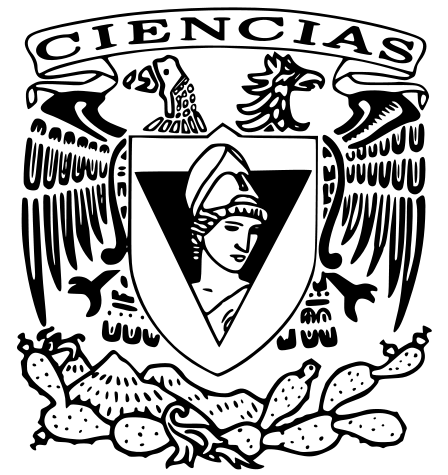
\includegraphics[scale=.19]{fac.png}}
\end{picture}

\begin{center}
\vspace*{0.2in}
{\fontsize{21}{21}\selectfont Universidad Nacional Autónoma de México}\\
\vspace*{0.2in}
{\fontsize{18}{18}\selectfont Facultad de Ciencias}\\
\vspace*{0.2in}
\begin{large}
{\fontsize{14}{14}\selectfont Laboratorio de Electromagnetismo} \\
\end{large}
\vspace*{0.2in}
\vspace*{0.2in}
\begin{Large}
\textbf{Práctica 4} \\
\textbf{ Capacitores, su funcionamiento, la capacitancia \\y la constante dieléctrica } \\
\end{Large}
\vspace{.7 cm}
Integrantes del equipo:\\
1) Alonso Barradas Luis Gustavo\\ 
2) Fragoso Alvarado Daniel\\ 
3) Rios Fematt Mildred Stephany\\ 
4) Robledo Ibarra Emiliano\\
\paragraph{}
\begin{figure}[H]
    \captionsetup{justification=centering,margin=2cm}
    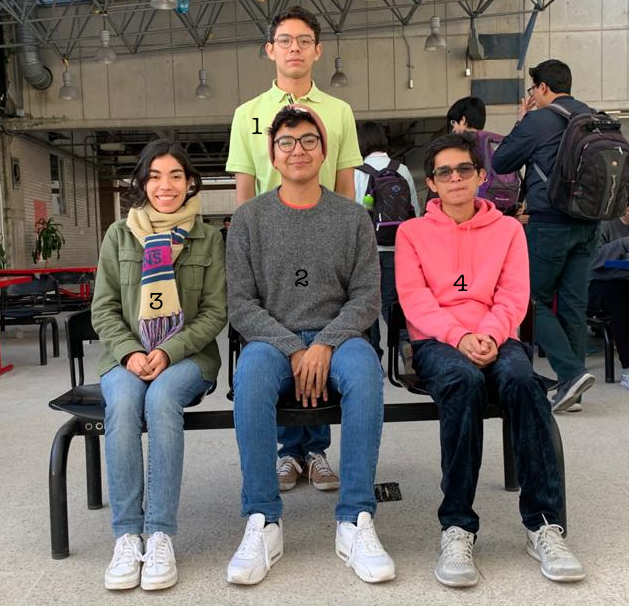
\includegraphics[scale=0.23]{uwu.jpg}
    \centering
\end{figure}
\rule{80mm}{0.1mm}\\
\begin{large}
Profesora:  Fís. Maris Sofía Flores Cruz.  \\
Ayudante: Miguel Ángel Amaya Reyes. \\
Fecha de entrega: Miercoles 11 de Marzo, 2020\\
\end{large}
\end{center}

\newpage

%------------------------------------


\begin{multicols}{2}

\section{Objetivos}
\begin{enumerate}
    \item Identificar las partes físicas que constituyen un capacitor, explicar su funcionamiento y analizar las ecuaciones lo describen.
    \item Para un arreglo de dieléctricos rígidos, medir la capacitancia de un capacitor y obtener el valor de la constante dieléctrica de diferentes medios eléctricos. 
    \item Analizar el comportamiento cualitativo de las gráficas de Capacitancia para distintos dieléctricos en película. %(papel, teflón y mica)  
\end{enumerate}

\section{Introducción}

%El principio que sigue un capacitor fue observado en 1745 con la invención de lo que hoy conocemos como \textit{Jarra de Leyden}, que es considerado el primer capacitor de la historia. La Jarra de Leyden consiste básicamente en una botella (jarra) de vidrio, que estaba forrada de papel metálico tanto dentro como fuera de la botella; además estaba cerrada por medio de un corcho por el que pasaba una cadena metálica conectada a un generador de cargas. Leyden observó que una vez se hiciera pasar carga eléctrica por medio de la cadena el frasco mantendría dos cargas iguales pero opuestas en equilibrio hasta que se conectaran con un cable que produjera una chispa o un choque \cite{articulo}.%

Se define como \textit{Capacitor} a un dispositivo que almacena energía eléctrica en un campo electrostático. Una aplicación de los capacitores es crear campos eléctricos, como el dispositivo de placas paralelas que produce el campo eléctrico casi uniforme que desvía los haces de electrones en un tubo de televisión o de un osciloscopio \cite{resnik2002}.

%Se puede definir de forma rápida a un \textit{Capacitor},como un dispositivo que almacena energía en un campo eléctrico %ME QUIEREN VER LA CARA DE ESTUPIDA? JAJAJA NO CREO QUE SEA UN CAMPO ELECTRICO...
%.

Un capacitor --básico-- está constituido por dos conductores paralelos separados entre ellos; con el espacio entre ellos ocupado por un dieléctrico\footnote{Un dieléctrico es un material aislante, es decir que no cuenta con cargas libres \cite{finn1999}}. A los conductores se les suele llamar \textit{placas} independientemente de su geometría. Cuando se conecta un capacitor a una fuente de voltaje, ésta ``envía'' electrones de una placa hacía la otra, logrando que la placa a la que le fue extraída los electrones posea carga positiva y a la que los adquirió, posea carga negativa. Al haber un dieléctrico de por medio, las cargas se terminan acumulando en las placas del capacitor debido a su incapacidad de atravesar el dieléctrico. Se dice entonces que: un capacitor está cargado cuando sus placas poseen cargas de igual valor y signo contrario. 
Si se desconecta la fuente de voltaje, las cargas acumuladas en la placas no tendrán hacía donde ``moverse", por lo que el capacitor queda cargado y almacenando energía eléctrica.



%la carga (negativa) que se genera intenta recorrer el circuito formado, pero ésta se detiene en en la placa del capacitor debido a la intervención del dialéctico, mientras que la otra placa se ve forzada a ceder la carga negativa, lo cual genera una acumulación de carga en ambas placas, de la misma magnitud pero de signo contrario; es entonces cuando se dice que un capacitor está "cargado" \cite{finn1999}.

Al cargar un capacitor, se hace pasar carga constante por un conductor, lo cual genera un potencial eléctrico proporcional a la carga que lo produce; entonces es normal pensar que el cociente de ambas --carga y potencial-- será una constante de proporcionalidad, que será necesaria para convertir la relación en una igualdad. Dicha constante es llamada \textit{Capacitancia}. Es decir, que la capacitancia de un conductor aislado se define por el cociente entre su carga y su potencial, y su unidad esta dada por el \textit{farad}  \footnote{Un farad se define como la capacitancia de un conductor aislado cuyo potencial, después de recibir una carga de un coulumb es de un volt.} ($1F=\frac{C}{V}$) \cite{finn1999}:
\begin{equation}
    C=\frac{Q}{V}
\end{equation}{}


Sin embargo, en una capacitor no sólo tenemos el sistema de un conductor, sino de dos con misma carga pero de signo opuesto. En ese caso, podemos extender el concepto de capacitancia si tomamos la diferencia de potencial entre ambos conductores, de tal forma que definamos la capacitancia del sistema como:  
\begin{equation}
    C=\frac{Q}{V_{1}-V_{2}} = \frac{Q}{\Delta V}
\end{equation}{}


Donde $V_{1}$ y $V_{2}$ son los potenciales generados por las cargas $Q$ y $-Q$ respectivamente \cite{finn1999}.

La capacitancia se ve afectada al modificar la distancia que hay entre las placas. Si suponemos que los conductores llegan a acercarse sin ser desconectados de la fuente de voltaje, entonces la diferencia de potencial se mantendrá constante; pero al disminuir la distancia, el campo eléctrico entre las placas aumentará, incrementando así el valor de la carga. Obteniendo como consecuencia un aumento en la capacitancia.
Ahora, si suponemos que los conductores se acercan sin estar conectados a la fuente de voltaje, entonces la diferencia de potencial disminuirá; pero no habrá cambio alguno en la carga del capacitor, ya que no hay una fuente de voltaje que permita un intercambio de carga, por lo que la capacitancia se verá de igual forma aumentada.

La capacitancia no sólo varía con la distancia entre las placas; en realidad es un factor geométrico, es decir que depende del tamaño, la forma y la separación de las placas, lo mismo que del dieléctrico que ocupa el espacio entre ellas; sin embargo, la capacitancia de un capacitor no depende de $\Delta V$ ni de $q$. \cite{resnik2002}.

Debido a la dependencia geométrica que existe, hay ``diferentes" tipos de capacitores de acuerdo a la geometría que siguen. La más fácil de estudiar, y la que se aborda a lo largo del documento, es el capacitor de \textit{Placas paralelas}, el cual como su nombre lo indica son dos planos paralelos (\textbf{Figura 1}). Bajo esta configuración podemos calcular la diferencia de potencial del sistema\footnote{Los cálculos para obtener dichas expresiones se anexan en el \textbf{Apéndice 2}}:
%LO CONSIDERO Innecesario
\begin{equation}
   \Delta{V}=\frac{Q}{A \epsilon_{0}} d
\end{equation}{}
y tenemos entonces que la capacitancia es (Griffiths):
\begin{equation}
    C=\frac{ \epsilon_{0} A}{d}
\end{equation}{}

Donde $A$ es el área de las placas. Observemos que estas expresiones se obtienen suponiendo que nos encontramos en el vacío, pero esto no ocurre, pues en un capacitor está de por medio un material dieléctrico.

Debido a la naturaleza eléctrica de éste, el dieléctrico hace que las moléculas que lo conforman se polaricen como efecto de las cargas presentes en las placas. Si la diferencia de potencial se mantiene constante, con ayuda de la fuente de voltaje, entonces el dieléctrico ocasionará un aumento de carga en el capacitor. Si la carga del capacitor se mantiene constante, al desconectar la fuente de voltaje, entonces al incorporar el dieléctrico al sistema, la diferencia de potencial se verá disminuida. Como consecuencia de ambos casos se obtiene un aumento en la capacitancia.

La presencia del dieléctrico aumenta la capacitancia por un factor $k_\epsilon$. 
\begin{equation}
C'=k_\epsilon C
\end{equation}

Donde $k_\epsilon$ es la denominada constante dieléctrica; la cual varía con el aislante empleado en el capacitor.

En un capacitor de placas paralelas con dieléctrico se tiene que:
\begin{equation}
C'=\frac{k_{\epsilon}\epsilon_{0}A}{d}
\end{equation}

%Es natural pensar que el campo eléctrico generado al exponerse a un dialéctico se ve disminuido. De hecho con el capacitor en el vacío, el campo eléctrico está dado por la ecuación: $ E=q / \epsilon_{0} A$. Cuando el dieléctrico está presente podemos pensar en un nuevo valor de $\epsilon_{0}$ que varia según el dieléctrico, digamos $\epsilon$ y
% PARA NADA DE ACUERDO

%que aminora el campo eléctrico por su presencia; pero esto hace que las placas adquieran nueva carga: $q^{\prime}$, de modo que el campo también cambia y esta dado por: $E^{\prime}=q^{\prime} / \epsilon A .$ Puesto que los campos han de ser iguales, podemos hacer $E^{\prime}=E$ y concluir que
%$$q^{\prime}=\frac{\epsilon}{\epsilon_{0}} q$$%

%Donde el cociente $\epsilon / \epsilon_{0}$ es la constante dieléctrica del material. La capacitancia con el dialéctico presente es entonces:$$C=\frac{\epsilon A}{d}$$

Esto sugiere un medio práctico para medir la constante dieléctrica de un material. Primero se medirá la capacitancia de un capacitor sin material entre las placas, %resultando:$$C_{0}=\frac{\epsilon_{0}A}{d}$$
luego llenamos el espacio entre las placas con el material que se está investigando y medimos la nueva capacitancia. Entonces tenemos despejando el área e igualando:
$$
\frac{C'}{C}=k_\epsilon
$$
Por consiguiente, el cociente entre las dos capacitancias da la constante dialéctica del material colocado entre las placas \cite{finn1999}.

\section{Desarrollo experimental}

Con ayuda de los siguientes materiales se obtuvieron las mediciones esenciales para la realización de la práctica:

%%% Lista de Materiales %%%
\setlist{nolistsep}
\begin{itemize}
     \item Multímetro Digital ($\pm3.0\%  + 5  \text{dígitos}$)
    \item Soporte para placas
    \item Pares de placas de aluminio circulares:
    \begin{itemize}
        \item De $(6.295 \pm 0.002) cm$ de radio
        \item De $(8.300 \pm 0.002) cm$ de radio
        \item De $(9.850 \pm 0.002) cm$ de radio
        \end{itemize}{}
    \item Cables conductores 
    \item Pinzas de presión
      \item Diferentes dieléctricos:
     \begin{itemize}
         \item Acrílico
         \item Vidrio
         \item Madera
         \item Papel
         \item Teflón
         \item Mica
     \end{itemize}{}
\end{itemize}{}

%%% Descripción del Montaje %%%

\begin{figure}[H]
    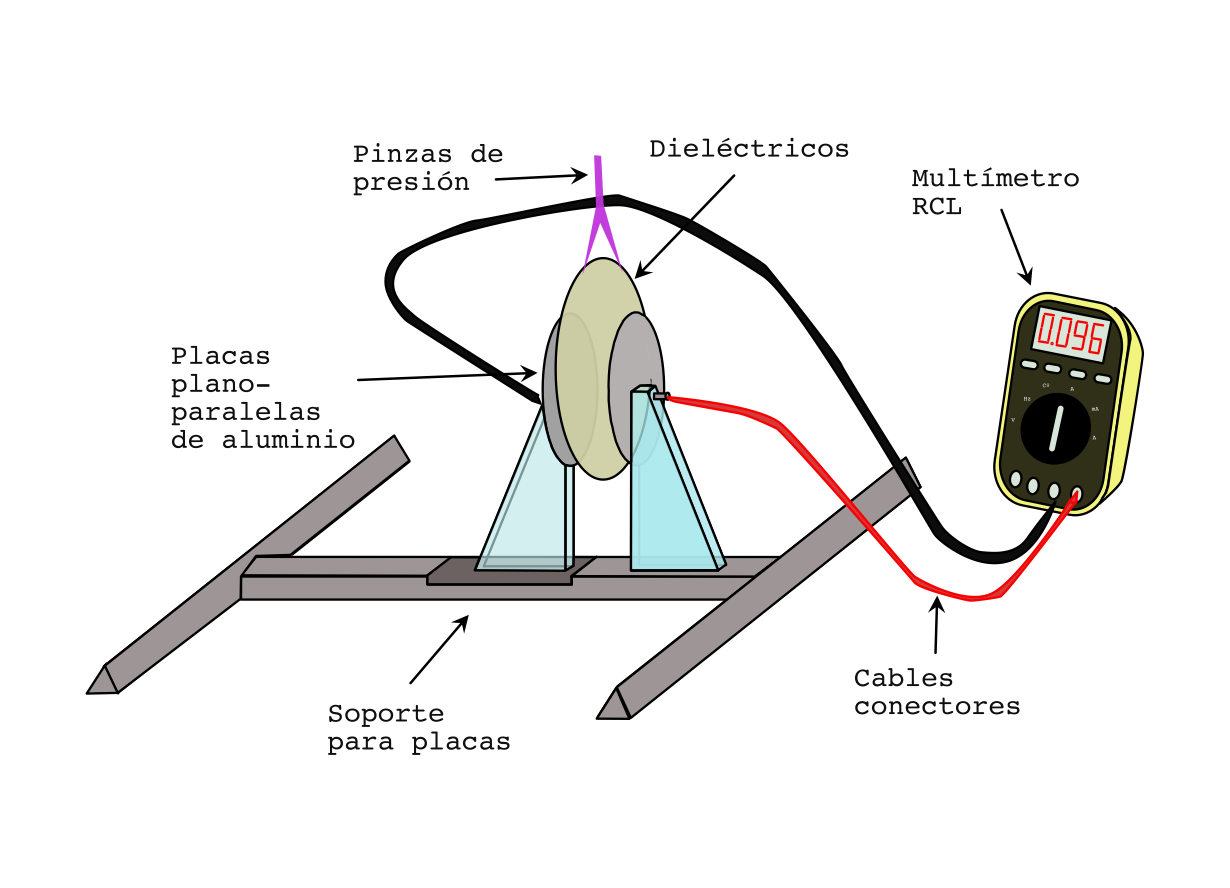
\includegraphics[scale=0.20]{Yanomegustaivonne1.png}
    \caption{Diagrama del arreglo experimental}
    \centering
\end{figure}
Durante la experimentación fueron ensamblados distintos capacitores, con la finalidad de observar cómo es que estos funcionaban al cambiar algún elemento de su estructura. Los elementos intercambiados durante este proceso fueron: el área de las placas, la distancia de separación y el dieléctrico entre ellas.
Los conductores empleados fueron pares de placas de aluminio con forma circular, donde el diámetro de cada par era distinto al de los demás. De igual forma, los dialécticos rígidos poseían forma de disco, y su diámetro era igual al de la placa empleada en cada distinto momento.

Como primera parte de la práctica, se llevó a cabo el cambio de dialéctico rígido entre las placas. 
Inicialmente fue colocado en el soporte el par de placas de aluminio que poseía mayor diámetro, y se escogió como primer dialéctico el disco de acrílico. Éste fue colocado entre las placas y ajustado por medio de pinzas de plástico, para evitar su posible deslizamiento sobre las placas. En seguida, se conectó el multímetro a cada placa por medio de dos cables conductores (\textbf{Figura 1}); así éste obtuvo un valor de la capacitancia para dicho dialéctico formado. 


\begin{figure}[H]
    \captionsetup{justification=centering,margin=2cm}
    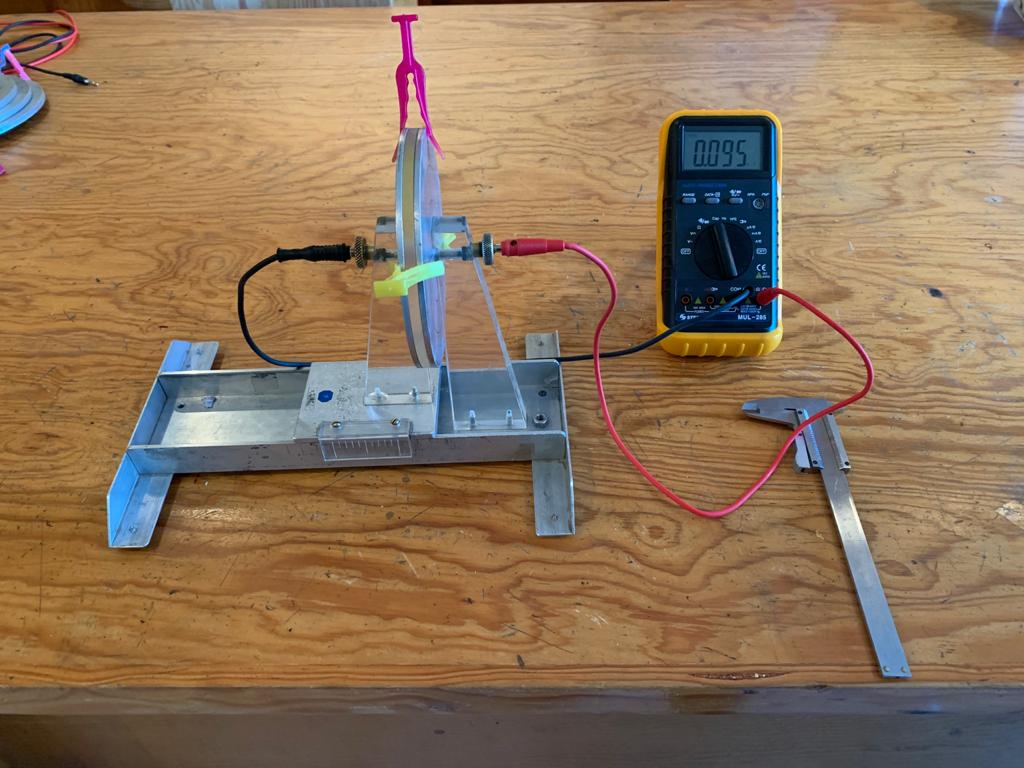
\includegraphics[scale=0.20]{adiosivana.jpeg}
    \caption{Foto del arreglo experimental}
    \centering
\end{figure}

Después de haber registrado el valor de la capacitancia con el primer dieléctrico rígido, se prosiguió a medir el valor de ésta al quitar el disco de acrílico; es decir que, nuevamente se midió la capacitancia con las mismas placas de aluminio, a la misma distancia que el ancho del disco del dialéctico retirado, considerando ahora como dieléctrico al aire entre las placas. Se registró el valor de la capacitancia obtenida por el multímetro. 
A continuación, se realizó el mismo procedimiento de ensamblaje (véase \textbf{Figura 2}) con los otros dos dieléctricos rígidos: disco de vidrio y disco de madera; de igual forma se registraron las capacitancias obtenidas al retirar los distintos dieléctricos del capacitor, de manera que el aire entre las placas hiciera el papel del dieléctrico empleado. Se registraron los valores obtenidos en los dos distintos casos. 

Como paso consecutivo, se prosiguió a medir la capacitancia obtenida al cambiar el radio de las placas conductoras. Se colocaron en el soporte de placas, un par de aluminio con un radio distinto al anterior, y siguiendo el proceso previo, se midieron las distintas capacitancias para los tres dieléctricos rígidos. Como consecuencia del cambio de las placas de aluminio, se eligieron discos de los tres materiales dieléctricos con los mismos radios que las placas tomadas en cada caso. Dicho proceso se repitió por tercera vez, siendo en total tres pares de discos estudiados; cada uno con tres dieléctricos distintos.

Como segunda parte de la práctica, se midieron las capacitancias de distintos dialécticos en películas. Para ello se empleó el simulador de Laboratorio de Capacitores de PhET™. 
En dicha sección, se tomaron a través de \cite{burb2007} las constantes dieléctricas del Teflón, del Papel y de la Mica. Siendo respectivamente: 2.1, 3.5 y 5; las cuales permanecieron fijas durante todo el proceso. Con estos tres distintos materiales dados, se analizó la dependencia de la capacitancia con la distancia entre las placas y el área que poseía el par de placas conductoras. 

Como primera parte del análisis, se modificaron las distancias entre las placas. Para esto se fijaron dos áreas de los materiales conductores: la primera de 100$mm^2$ y la segunda de $400mm^2$. En seguida, se analizó el comportamiento cualitativo de las gráficas obtenidas.  Véase \textbf{Figura 5}.

Como segundo análisis, se fijaron las distancias de 5mm y de 10mm, y se procedió a variar el área de las placas. En seguida, se analizó el comportamiento cualitativo de las gráficas obtenidas (\textbf{Figura 3}).

Ambos análisis fueron realizados para cada distinto dieléctrico en película. 

%%% Descripción del Procesamiento de datos %%%


\section{Resultados, análisis y discusión}
\paragraph{El funcionamiento del capacitor. } 
Como ya sabemos, un capacitor está compuesto por dos conductores separados por un aislante (o vacío). En nuestro caso particular las placas de aluminio sirvieron como conductores. Observemos que la placa derecha del capacitor se conectó a la terminal positiva del multímetro mediante un cable conductor; del mismo modo, la placa izquierda se conectó a la terminal negativa (\textbf{Figura 3}). Lo que ocurrió a continuación fue que tanto la placa derecha, como la terminal del multímetro, de la cual estaba conectada, presentaban un mismo potencial eléctrico. Sucediendo lo mismo con la placa izquierda y la terminal negativa. Esta diferencia de potencial entre las placas, produjo un campo eléctrico, el cual es esencialmente uniforme gracias a que la separación entre placas que es lo suficientemente pequeña, comparada con el área de las placas; razón por la cual sólo se tomaron medidas a ($0.1<d<1.0$)cm. Esto produjo que los conductores se cargaran uniformemente de manera positiva y negativa en sus respectivas superficies.

%, produce un campo eléctrico, el cual es esencialmente uniforme
%gracias a la geometría plana de las placas, si la separación entre placas es lo suficientemente pequeña,  comparada con el área de las placas, razón por la cual sólo se tomaron medidas a $0.1<d<1.0$cm. Esto hace que los conductores se carguen  uniformemente de manera positiva y negativa en sus respectivas superficies.
Podemos observar de la ecuación \textbf{(6)} que la capacitancia de un capacitor únicamente depende del área de las superficies, de la distancia entre placas y de la constante dieléctrica. 
Al ser directamente proporcional al área, nos indica que entre más grande sea el área de las placas, la capacitancia irá en aumento. Lo cual tiene sentido físico; ya que entre más grande sea el área que poseen las placas, mayor será su capacidad de almacenar cargas. En el caso de la distancia entre las placas, la capacitancia es inversamente proporcional a ella, revelando así que, la disminución de la distancia entre los conductores traerá como resultado un valor mayor en la capacitancia. 

%Como es directamente proporcional al área, esto indica que entre mayor área tengan las placas, mayor será su capacitancia. Lo cual tiene sentido físico, porque a mayor área significa que habrá mayor capacidad de almacenar carga; mientras que para la distancia es inversamente proporcional, lo que quiere decir que a menor distancia, la capacitancia incrementará. 

\paragraph{Dieléctricos Rígidos}

Los siguientes datos muestran las mediciones obtenidas de la capacitancia (C') al tener distintos dieléctricos rígidos en un capacitor. Como resultado próximo se obtiene el valor de la constante dieléctrica ($k_\epsilon$).
En un mismo espacio se muestra el dieléctrico empleado, la capacitancia obtenida al tenerlo en el capacitor y el valor obtenido después de retirarlo.

Para las diferentes áreas de los discos de aluminio, se tienen las siguientes tablas:




\begin{table}[H]
\begin{center}
\begin{tabular}{ |c|c|c|c|c| } 
\hline
Material   & Distancia [cm]   & Cap. [pF] & $k_\epsilon$ \\
\hline

Acrílico  & $0.585 \pm 0.002$  & $53\pm7$  &$3.02 \pm 0.01 $ \\
Aire      &                   & $25 \pm 6$ & $ 1.320 \pm 0.006$\\
\hline

Vidrio  &  $0.580 \pm 0.002$   & $90.\pm8$ & 5.40 $\pm$ 0.03\\
Aire   &                       & $24 \pm 5$ &1.297 $\pm$ 0.006 \\
\hline

Madera & $0.525 \pm 0.002$ & $68\pm7$  & 3.61 $\pm 0.02$\\
Aire &                      &$28 \pm 6$ &$1.250\pm 0.006$ \\

\hline

\end{tabular}
\end{center}

\caption{Datos presentados para 
\textbf{Radio: $(6.295 \pm 0.002) cm$}}
\label{Tabla 1}
\end{table}
%%%%%%%%%%%%%%%%%%%%%%%%%




\begin{table}[H]
\begin{center}
\scalebox{0.9}{
\begin{tabular}{ |c|c|c|c| } 
\hline
Material   & Distancia [cm]   & Cap. [pF] & $k_\epsilon$ \\
\hline

Acrílico  & $0.600 \pm 0.002$  & $96\pm8$ & $2.83 \pm 0.02$  \\
Aire      &                  & $42 \pm 6$ & $1.333 \pm 0.008$ \\

\hline

Vidrio &  $0.590 \pm 0.002$  &  $175\pm10$ & $4.76 \pm0.03$   \\
 Aire &                      & $42 \pm 6$ & $1.258\pm0.008$ \\

\hline

Madera &    $0.570 \pm 0.002$      & $121\pm9$  & $3.25 \pm0.02$ \\
Aire &                       & $42 \pm 6$  &  $1.340\pm0.008$\\

\hline

\end{tabular}
}
\end{center}
\caption{Datos presentados para \textbf{Radio: $(8.300 \pm 0.002) cm$}}
\label{Tabla 1}
\end{table}


%%%%%%%%%%%%%%%%%%%%%%%%%%%%%%%%%%%%%%%%%%%%%%%%%%%%%%%%%%%%%%%%%%


%%%%%%%%%%%%%%%%%%%%%%%%%%%%%%




\begin{table}[H]
\begin{center}
\scalebox{0.9}{
\begin{tabular}{ |c|c|c|c| } 
\hline
Material   & Distancia [cm]   & Cap. [pF] & $k_\epsilon$ \\
\hline

Acrílico &  $0.600\pm0.002$  & $122 \pm 9$  &  $2.71 \pm0.01$  \\
Aire     &                     &   $56\pm7$       & $1.247\pm0.004$  \\
\hline

Vidrio& $0.595 \pm 0.002$  & $232\pm12$ & $5.12 \pm0.01$  \\
 Aire &                     & $53 \pm 7$ & $1.170\pm0.004$  \\

\hline

Madera  & $0.570 \pm 0.002$   & $142\pm9$ & $3.00 \pm 0.02$  \\
Aire &                         & $52 \pm 7$ & $1.100 \pm 0.005$\\

\hline

\end{tabular}
}
\end{center}
\caption{Datos presentados para 
\textbf{Radio: $(9.850 \pm 0.002) cm$}}
\label{Tabla 1}
\end{table}

De la tablas anteriores, se puede observar una característica relacionada a los valores de la capacitancia, obtenida para el aire en cada caso. Y es que, en los tres pares de discos empleados, al retirar el aislante utilizado, la capacitancia tuvo un valor semejante para los diferentes dieléctricos. En primera instancia se hace visible una reducción de la capacitancia al retirar el aislante. Como consecuente de esto, se puede notar que los datos de ésta se asemejan entre sí; pero al calcular con ello, el valor de la constante dieléctrica del aire es cuando se percibe aún más tal parecido. De esta manera, observamos que el aire presenta una constante dieléctrica cercana a uno, pues la tendencia de estos valores es hacia a $1.258\pm0.006$.

En lo que a valores de capacitancia se refiere es necesario mencionar que para los tres radios acordados se guarda un mismo orden: el vidrio siempre tiene mayor capacitancia, seguido por la madera, después el acrílico y por último el aire. Es así como se puede advertir que la capacitancia es dependiente del material aislante; cosa que es también observable en el resultado realizado al obtener la constante dieléctrica $k_\epsilon$, pues éste guarda el mismo orden antes mencionado. Es gracias a este mismo orden que, sabemos que cada material es distinto en cuanto a capacitancia se refiere; y cómo esta propiedad de ellos ayuda en mayor o menor medida a que el capacitor almacene energía eléctrica.

Otro aspecto marcado que podemos notar es la relación que existe entre las áreas de las placas y la capacitancia obtenida. Al aumentar el radio de los discos de aluminio, y por ende el área de estos, la capacitancia de todos los dieléctricos se vio incrementada. Tal característica se hizo notaria al pasar desde el par de discos más pequeños (referente al área), hasta los más grandes. Esta propiedad nos hace pensar que el área de las placas es un factor importante en cuanto a la capacitancia.


%Lo que se puede observar de las tablas anteriores es que para todo radio probado, al retirar el dieléctrico utilizado la capacitancia se reduce  pero no solamente se reduce sino que llega a un valor semejante con cada dieléctrico, que al utilizarlo para calcular la constante de dieléctrica arroja valores concordantes entres sí. De esta manera, observamos que el aire tiene una capacitancia cercana a uno pues la tendencia de estos valores es hacia a $1.258\pm$; esto implica que no solamente se está encontrando que el aire funciona como dieléctrico en un capacitor pues en suma se calculó que tiene una constante dieléctrica cuyo intervalo concuerda con el que se reporta en la literatura. 
%Otro aspecto marcado que podemos notar es que entre mayor sea el radio de las placas y, en consecuencia, el área de estas, el valor de la capacitancia medida para un dieléctrico incrementa, además  esto ocurre para los tres valores de los radios probados lo cual nos hace pensar que el área de las placas es un factor importante en cuanto a la capacitancia que tiene el arreglo.
%En lo que a valores de capacitancia refiere es necesario mencionar que para los tres radios acordados siempre guardan un orden, a saber: el vidrio siempre tiene mayor capacitancia, le sigue la madera, después el acrílico y por último el aire. Así, podemos observar que la capacitancia es dependiente del material y esto es también observable en el resultado realizado para obtener la constante dieléctrica $k_\epsilon$ pues guarda el mismo tipo de orden antes mencionado. Gracias a dicho orden, sabemos que cada material es distinto en cuanto a capacitancia refiere, y observamos como el vidrio cuenta con la mayor capacitancia en los materiales elegidos lo que implica una mayor efectividad de almacenamiento de carga.

\paragraph{Dieléctricos de Película}

%A continuación las tablas de los dieléctricos por láminas para el radio $r = (9.850 \pm 0.002) cm$:

%\begin{table}[H]
 % \centering
 %   \begin{tabular}{|c|c|c|} \hline
 %   Láminas & Separación [cm] & Capacitancia [nF] \\ \hline
 %   12    & 0.335 $\pm 0.002$ & 0.177 $\pm 0.010$ \\
 %   11    & 0.294 $\pm 0.002$ & 0.187 $\pm 0.011$ \\
  %  10    & 0.270 $\pm 0.002$ & 0.202 $\pm 0.011$ \\
  %  9     & 0.260 $\pm 0.002$ & 0.212 $\pm 0.011$ \\
 %   8     & 0.250 $\pm 0.002$ & 0.229 $\pm 0.011$ \\
 %   7     & 0.235 $\pm 0.002$ & 0.246 $\pm 0.012$ \\
 %   6     & 0.160 $\pm 0.002$ & 0.247 $\pm 0.012$ \\
 %   5     & 0.140 $\pm 0.002$ & 0.264 $\pm 0.013$ \\
 %   4     & 0.120 $\pm 0.002$ & 0.313 $\pm 0.014$ \\
 %   3     & 0.100 $\pm 0.002$ & 0.403 $\pm 0.017$ \\
 %   2     & 0.090 $\pm 0.002$ & 0.57 $\pm 0.02$ \\ \hline
 %   \end{tabular}%
 %   \caption{Capacitancia para láminas de cartulina}
 % \label{tab:addlabel}%
% \end{table}%

%La tabla anterior muestra cómo para menores distancias la capacitancia se reduce; de manera que podemos observar como la capacitancia además de depender del material y el área de las placas, depende a su vez de la separación que tienen las mismas placas que lo forman. Siguiendo este razonamiento y comparando la distancia del vidrio es sencillo ver que comparando la cartulina con el vidrio, este último cuenta con una mayor capacitancia pues como se observa en la tabla, si tuviésemos una menor distancia se esperaría un mayor valor y mucho mayor al de la cartulina. 






%%%%%%%%%%%%%%%%%%%%%ANÁLISIS DE gráficas

\paragraph{Capacitancia en función del área:}
\begin{figure}[H]
    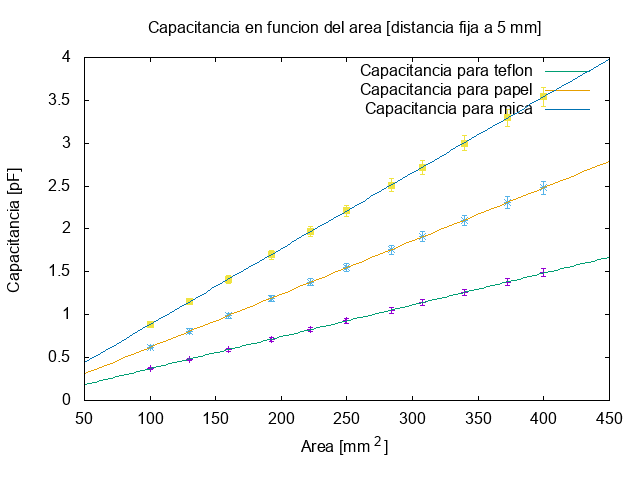
\includegraphics[scale=0.43]{CA100.png}
    \caption{Gráfica que muestra a la capacitancia en función del área, fijándola a una distancia de 5mm}
    \centering
\end{figure}
\begin{figure}[H]
    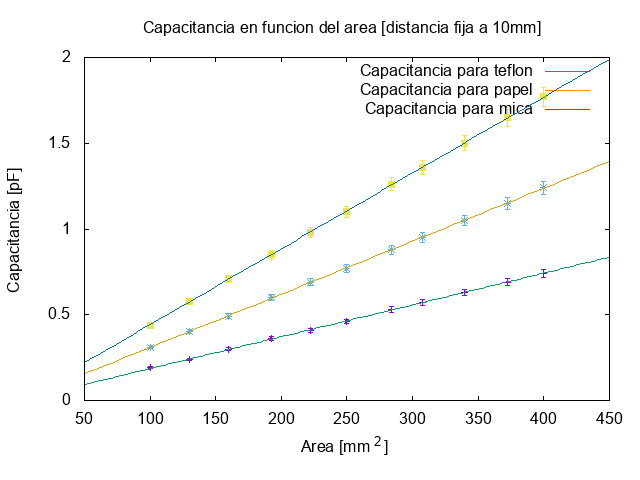
\includegraphics[scale=0.45]{CA400.png}
    \caption{Gráfica que muestra a la capacitancia en función del área, fijándola a una distancia de 10mm}
    \centering
\end{figure}

Al analizar ambas gráficas, se hace notorio que el área es directamente proporcional a la capacitancia; es decir que, se encontró una relación lineal entre ambos valores, característica que era esperada después de haber visto tal resultado en los dieléctricos rígidos. De igual forma, al examinar las dos gráficas, se presenció una relación entre la capacitancia obtenida y el material usado como dieléctrico. Como los valores de las constantes dieléctricas fueron dadas en un inicio (5 para la Mica, 3.5 para el Papel y 2.1 para el Teflón), se contempla, debido a estos valores dados, como es que ellos influyen en la capacitancia obtenida. Siendo así que en las gráficas se señale una mayor capacitancia para la Mica, seguida del papel y por último, el Teflón.

Contemplemos cómo a medida que el área crece, los valores de la capacitancia se alejan entre sí para los diferentes dieléctricos estudiados (obsérvese como ejemplo \textbf{Figura 3}). Esto nos dice que, con un área mayor para las placas y utilizando un aislante con una constante dieléctrica mayor, se  esperaría observar una capacitancia más grande en valor, a comparación de utilizar un capacitor con área menor y un aislante con un valor de constante dieléctrica igual o menor al anterior.

%Observemos que en este caso, se hace notorio que el área es directamente proporcional a la capacitancia, es decir se esperaba encontrar una relación lineal.
%Cuando la distancia fue mínima (en \textbf{Figura 3}), se observa como a medida que el área crece, los valores de la capacitancia se alejan entre sí para los diferentes dieléctricos que se analizaron, esto quiere decir que a mayor área y utilizando un dieléctrico con un valor dieléctrico alto, esperaríamos observar una capacitancia mayor, lo cual  

Haciendo la comparación entre las dos gráficas, donde la distancia ocupada en \textbf{Figura 4} es el doble que en \textbf{Figura 3}, es visible que en ambas se mantiene la misma relación lineal de la capacitancia con el área de las placas; pero no es lo único, sino que, también se observa que en el caso en que la separación fue de 10mm, la capacitancia obtenida se mostró como la mitad del valor obtenido al tener una separación de 5mm. Es decir que, al aumentar a distancia entre las placas por un factor de 2, la capacitancia se vio reducida a la mitad.

%Algo importante que recalcar en \textbf{Figura 4}, es que la distancia que se ocupó fue de 10mm a diferencia de nuestra primer distancia la cual fue de 5mm, lo que quiere decir que aumentamos al doble nuestro valor de la distancia, y lo que se observa es que el valor de la capacitancia, en vez de aumentar disminuyó en un factor de 2,
%dando a observar el comportamiento de la distancia el cual es inversamente proporcional al valor de la capacitancia y si esto es así, al momento de fijar el área se esperaría encontrar una relación de la forma $C(d)=\frac{a}{d}$

\paragraph{Capacitancia en función de la distancia:}

\begin{figure}[H]
    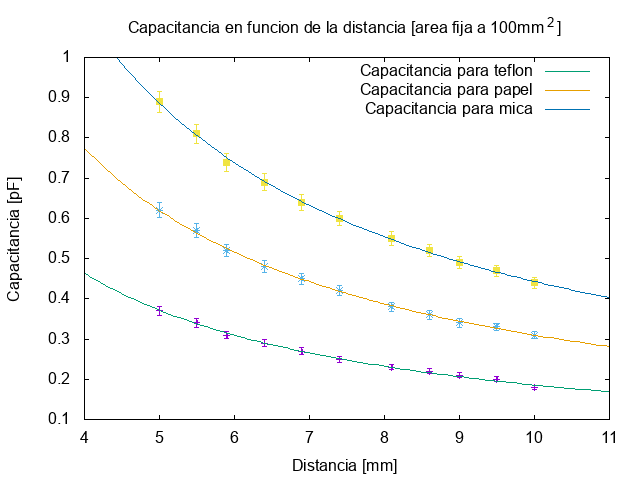
\includegraphics[scale=0.5]{Cd100.png}
    \caption{Gráfica que muestra a la capacitancia en función de la distancia , fijándola a un área mínima de 100$mm^2$}
    \centering
\end{figure}


\begin{figure}[H]
    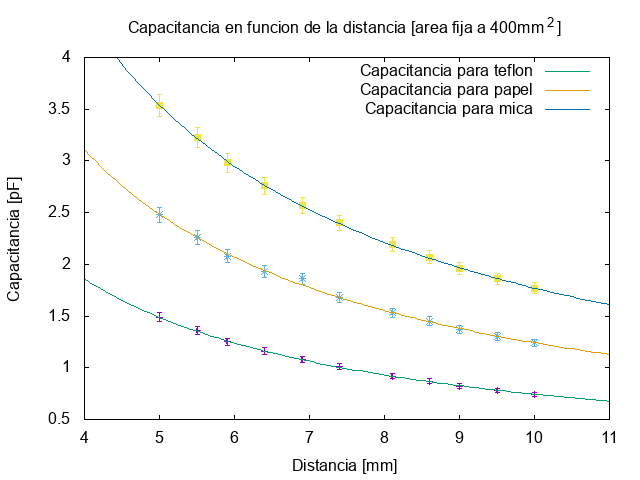
\includegraphics[scale=0.5]{QUIEROSERTUYOIVONNE.png}
    \caption{Gráfica que muestra a la capacitancia en función de la distancia , fijándola a un área máxima de 400mm}
    \centering
\end{figure}
%%%CHORRO MAREADOR DE LAS PUTAS GRÁFICAS

En ambas gráficas es apreciable cómo la capacitancia disminuye conforme la distancia va en aumento. En el caso de la \textbf{Figura 5} se tienen valores de capacitancia menores que en los de \textbf{Figura 6}, esto es únicamente debido a que el área de las placas fijada en la primera, es menor por un factor de 4 que en la segunda. Y cómo se vio en las gráficas que muestran la relación de la capacitancia con el área de las placas, es ésta una relación directamente proporcional. 

Recordemos que de las gráficas anteriores (\textbf{Figura 3} y \textbf{Figura 4}) también se pudo encontrar una relación entre la capacitancia y la separación entre placas. Donde al haber un aumento de la última, la capacitancia se veía disminuida. Esta observación, junto con el análisis de la \textbf{Figura 5} y \textbf{Figura 6}, nos lleva a pensar que existe una relación inversamente proporcional entre la capacitancia y la distancia; entonces, al momento de fijar el área, se pudo comprobar que la distancia es inversamente proporcional a la capacitancia.

Examinando estas gráficas de la capacitancia en función de la distancia,
se encuentra que la función se comporta de manera hiperbólica; justo como era lo esperado. 

Por último, al igual que en la relación anterior, en ambas gráficas se mostró una dependencia de la capacitancia con el material aislante, dispuesto en el capacitor.

%%%Discusión 1 y discusión 2

Veamos que para la primera sección se obtuvieron los siguientes resultados de la constante dieléctrica:

 % Table generated by Excel2LaTeX from sheet 'Hoja1'
 \begin{table}[H]
   \centering
     \begin{tabular}{|c|c|c|} \hline
     Acrílico & Vidrio & Madera \\ \hline
     
     3.02 $\pm$ 0.01    & 5.40 $\pm$ 0.03    &   3.60 $\pm$ 0.02 \\ \hline
     
    2.83 $\pm$ 0.02    & 4.76 $\pm$ 0.03     &    3.25 $\pm$0.02 \\ \hline
    
     2.72 $\pm$ 0.01   & 5.12 $\pm$ 0.01     &     3.00 $\pm$ 0.2 \\ \hline
     \end{tabular}%
   \label{tab:addlabel}%
    \caption{En la primer fila se muestra los datos del radio 1, y análogamente para los valores consecutivos }
 \end{table}%
Los cuales son valores que son cercanos entre sí, es decir que ninguno sobrepasa a otro en magnitud 1, a pesar de que al tomar en cuentas los decimales y la incertidumbre obtenida para cada constante estos sí presentaban una diferencia. Ésta se le puede atribuir a variaciones en los materiales utilizados; a pesar de tener materiales que se supone son iguales, como dos pedazos de madera. Estos presentan ciertas diferencias entre ellos, como se pudo haber dado el caso de una abolladura que cambia en un pequeño factor la densidad en tal región; por lo tanto, la constante dieléctrica no tendría por qué ser la misma, y esa diferencia se hace notoria en los decimales.
Para la segunda sección, se logró observar la relación que mantiene la Capacitancia con la distancia y el área, pudiendo comprobar que ésta es directamente proporcional al área e inversamente proporcional a la distancia.
\section{Conclusiones}

En la práctica se plantearon tres objetivos principales. En el cumplimiento del primero, se buscó hacer un análisis completo de nuestro sistema. Apoyándonos de la teoría, que nos indica la estructura de un capacitor básico, identificamos adecuadamente las partes que lo componen: siendo las placas paralelas de aluminio, los conductores; y el multímetro como la fuente de voltaje.
Además de esto, se buscó ver bajo que suposiciones las ecuaciones que describen su funcionamiento eran validas. En este caso, se reconoció que una distancia relativamente menor a la magnitud del área, era necesaria para inferir que el campo eléctrico actuando en el capacitor, era constante en todos los puntos de las placas. Y de tal forma, obtener de una manera más sencilla el cálculo de la capacitancia. 
En el momento que se fueron calculando los distintos valores de capacitancia para cada arreglo diferente del capacitor, se encontró la ligada dependencia de la capacitancia con la geometría del sistema, y con el tipo de aislante usado. Se apreció en cada experimento realizado, que la capacitancia aumentaba en forma proporcional al crecer el área de las placas; y que disminuía al crecer la separación entre las mismas placas. Una vez obtenida la capacitancia en el caso de los dieléctricos rígidos, se calculó el valor de la constante dieléctrica de cada aislante. Como consecuente de esto, se advirtió que el material con una constante dieléctrica mayor, que en comparación de las demás, poseía una capacitancia más grande. Dicho lo anterior, es como se pudo concluir que para el caso de dieléctricos rígidos, el vidrio a comparación de los demás materiales aislantes, ayudó en mayor grado al almacenamiento de energía en el capacitor; mientras que en los dieléctricos de película, la mica fue el material que mostró mayor contribución a la capacitancia. Si comparamos estos dos últimos dieléctricos, podemos llegar a la conclusión que, en la practica conviene más utilizar dieléctricos de película; ya que estos permiten a que la distancia entre placas sea menor, debido a su grosor. Más aún, en nuestro caso particular, la constante dieléctrica de la mica, resultó mayor a la de todos los demás materiales empleados en la práctica, dando así un valor superior al del vidrio, en cuanto a capacitancia se refiere.
%%%%%%%%%%%%%%%%%%%%%%%%%%%%%%%%%%%%%%%%%%%%

%%%%%%%%%%%%%%%%%%%%%%%%%%%%%%%%%%%%%%%%%%%%%%%%
Durante el desarrollo del experimento, los datos se obtuvieron relativamente con facilidad; aún así, se presentaron ciertos problemas que evitaron una mejor adquisición de ellos. Así pues, se proponen dos mejoras para la realización del experimento: la primera de ellas sería el trabajar con materiales nuevos, esto debido a que los dieléctricos utilizados, podían llegar a presentar abolladuras o pequeñas fisuras, que en la práctica no permiten suponer que la densidad de tal material es uniforme, lo que nos lleva a cometer errores sistemáticos al calcular su constante dieléctrica. Otra mejora que se propone es el poder fijar las bases sin la necesidad de utilizar pinzas de presión; ya que tal como su nombre lo dice, ejercen cierta presión al material, de manera que cuando se retiran y se procede a hacer la medición de la distancia, ésta suele tener un pequeño cambio y el error sistemático depende del material, en este caso, de que tan compresible sea dicho material.
Como se vino mencionando a lo largo del presente documento, una de las propiedades más significativas de los capacitores es el poder almacenar cargas; por lo tanto entre sus múltiples aplicaciones, las más significativas son baterías, memorias, y fuentes de alimentación.


\nocite{*}
\bibliographystyle{apacite}
\bibliography{mybib}
\appendix
\textbf{Apendice I}
\paragraph{Cálculo de incertidumbres}

Para obtener la incertidumbres de la capacitancia se utilizó la exactitud que nos proporcionaba el manual del multímetro, el cual era de ($\pm$3\% + 5 Dígitos).


Para la obtención de la incertidumbre de los siguientes datos, se utilizó la ecuación de propagación de incertidumbre \cite{bevi2002}.


Para el área de las placas circulares, de la ecuación $A=\pi (r_2^2-r_1^2)$, le asociamos la incertidumbre 

$\sigma_A=2\pi \sigma_r\sqrt{r_1^2+r_2^2}$ .

Para la constante dieléctrica de los materiales rígidos, de (\textbf{Equation 6}), le asociamos la incertidumbre:
$$\sigma_k=\sqrt{\left(\sigma_A \frac{\partial k}{\partial A}\right)^2+\left(\sigma_C \frac{\partial k}{\partial C}\right)^2+\left(\sigma_d \frac{\partial k}{\partial d}\right)^2}$$
Después de realizar las derivadas correspondiente y al tratar de simplificar términos, llegamos a la siguiente expresión:
$$\sigma_k=\frac{Cd}{A\epsilon_0 }\sqrt{\left(\frac{\sigma_A}{A}\right)^2+\left(\frac{\sigma_C}{C}\right)^2+\left(\frac{\sigma_d}{d}\right)^2}$$

Para los datos obtenidos mediante el simulador, dado que no conocíamos la manera en que éste calculaba dichos datos, se le asoció las incertidumbres previamentes descritas en el apéndice.

\end{multicols}
\end{document}



%\begin{table}[H]
%\begin{center}
%\scalebox{0.9}{%
%\begin{tabular}{ |c|c|c|c| } 
%\hline
%Material   & Distancia [cm]   & Cap. [pF] & Cte. dieléctrica \\
%\hline

%\multirow{3}{4em}{Acrílico \\ Aire} &  & \multirow{3}{4em}{$96\pm8$ \\
%$42 \pm 6$} & \multirow{3}{4em}{$2.826 \pm 0.02$ \\ $1.333 \pm 0.008$}\\ 
%& $0.600 \pm 0.002$ &  &\\ 
%&  &  & \\ 
%\hline

%\multirow{3}{4em}{Vidrio \\ Aire} &  & \multirow{3}{4em}{$175\pm10$ \\
%$42 \pm 6$} & \multirow{3}{4em}{$4.76 \pm0.03$ \\ $1.258\pm0.008}$\\ 
%& $0.590 \pm 0.002$ &  &\\ 
%&  &  & \\ 
%\hline

%\multirow{3}{4em}{Madera \\ Aire} &  & \multirow{3}{4em}{$121\pm9$ \\
%$42 \pm 6$} & \multirow{3}{4em}{$3.25 \pm0.02$ \\ $1.340\pm0.008$}\\ 
%& $0.570 \pm 0.002$ &  &\\ 
%&  &  & \\ 
%\hline

%\end{tabular}
%}
%\end{center}
%\caption{}
%\label{Tabla 1}
%\end{table}




%\begin{table}[H]
%\begin{center}
%\scalebox{0.9}{%
%\begin{tabular}{ |l|l|l|l|l| } 
%\hline
%Material   & Distancia [cm]   & Cap. [pF] & Constante Dieléctrica \\
%\hline

%\multirow{3}{4em}{Acrílico \\ Aire} &  & \multirow{3}{4em}{$53\pm7$ \\
%$25 \pm 6$} & \multirow{2}{}{$3.02 \pm 0.01 $\\$ 1.320 \pm 0.006$}\\ 
%& $0.585 \pm 0.002$ &  &\\ 
%&  &  & \\ 
%\hline

%\multirow{3}{4em}{Vidrio \\ Aire} &  & \multirow{3}{4em}{$90.\pm8$ \\
%$24 \pm 5$} & \multirow{2}{4em}{5.40 $\pm$ 0.03\\ 1.297 $\pm$ 0.006}\\ 
%& $0.580 \pm 0.002$ &  &\\ 
%&  &  & \\ 
%\hline

%\multirow{3}{4em}{Madera \\ Aire} &  & \multirow{3}{4em}{$68\pm7$ \\
%$28 \pm 6$} & \multirow{3}{4em}{3.61 $\pm 0.02$\\ $1.25\pm 0.006$}\\ 
%& $0.525 \pm 0.002$ &  &\\ 
%&  &  & \\ 
%\hline

%\end{tabular}
%}
%\end{center}
%\caption{}
%\label{Tabla 1}
%\end{table}




%\begin{table}[H]
%\begin{center}
%\scalebox{0.9}{%
%\begin{tabular}{ |c|c|c|c| } 
%\hline
%Material   & Distancia [cm]   & Cap. [pF] & $k$ \\
%\hline

%\multirow{3}{4em}{Acrílico \\ Aire} &  & \multirow{3}{4em}{$122\pm9$ \\
%$56 \pm 7$} & \multirow{3}{4em}{$2.717\pm0.01$ \\ $1.247\pm0.0$}\$\ 
%& $050.600 \pm 0.002$ &  &\\ 
%&  &  & \\ 
%\hline

%\multirow{3}{4em}{Vidrio \\ Aire} &  & \multirow{3}{4em}{$232\pm12$ \\
%$53 \pm 7$} & \multirow{3}{4em}{$5.125\pm0.01$ \\ $1.170\pm0.004$}\\ 
%& $0.595 \pm 0.002$ &  &\\ 
%&  &  & \\ 
%\hline

%\multirow{3}{4em}{Madera \\ Aire} &  & \multirow{3}{4em}{$142\pm9$ \\
%$52 \pm 7$} & \multirow{3}{4em}{3.005 \\ 1.100}\\ 
%& $0.570 \pm 0.002$ &  &\\ 
%&  &  & \\ 
%\hline

%\end{tabular}
%}
%\end{center}
%\caption{}
%\label{Tabla 1}
%\end{table}


\textbf{Radio: $(8.300 \pm 0.002) cm$}

\begin{table}[H]
\begin{center}
\begin{tabular}{ |c|c|c|c| } 
\hline
Material   & Distancia [cm]   & Cap. [pF] & $k$ \\
\hline

Acrílico& $0.600 \pm 0.002$    & $96\pm8$ & $2.826 \pm 0.02$  \\
Aire    &                      & $42 \pm 6$ & $1.333 \pm 0.008$ \\

\hline

Vidrio  &  $0.590 \pm 0.002$  & $175\pm10$ & $4.76 \pm0.03$ \\
 Aire  &                      & $42 \pm 6$ & $1.258\pm0.008$ \\

\hline

Madera  & $0.570 \pm 0.002$  & $121\pm9$   & $3.25 \pm0.02$  \\
 Aire   &                     & $42 \pm 6$ &  $1.340\pm0.008$ \\
\hline

\end{tabular}

\end{center}
\caption{}
\label{Tabla 1}
\end{table}



